%% LyX 2.0.4 created this file.  For more info, see http://www.lyx.org/.
%% Do not edit unless you really know what you are doing.
\documentclass[english]{article}
\usepackage[T1]{fontenc}
\usepackage[utf8]{luainputenc}
\usepackage{graphicx}
\usepackage{babel}
\begin{document}

\title{Analysis of 2012 Beamtest }

\maketitle

\section{Event selection}


\subsection{Time analysis}


\subsection{Seed Analysis}


\subsubsection{Hits tagging}

Hits are separated in 3 categories:
\begin{itemize}
\item ISOLATED= The hit has no neighbours in a 9 cm radius sphere
\item EDGE = The hit belongs to a track segment in a 9 cm radius sphere
\item CORE= all other hits
\end{itemize}
Each hit defines a neighbouring sphere of 9 cm and a principal component
anlysis is done on all neighbours. The ratio w of the 2 principal
axis is then used to tag the hit.
\begin{itemize}
\item w=0 → less than 3 neighbours, the hit is ISOLATED
\item w < 0.3 → the second axis is small, most probably hits are aligned
along the first axis, the hit is an EDGE one.
\item w > 0.3 , the hit is in the CORE of the shower.
\end{itemize}
The figure \ref{fig:Ratio-of-L2/L1}shows the distribution of w for
all the hits of a 60 GeV pion run. The 3 categories clearly exhibits.
On figure the same ratio is shown for preselected muon candidates

\begin{figure}
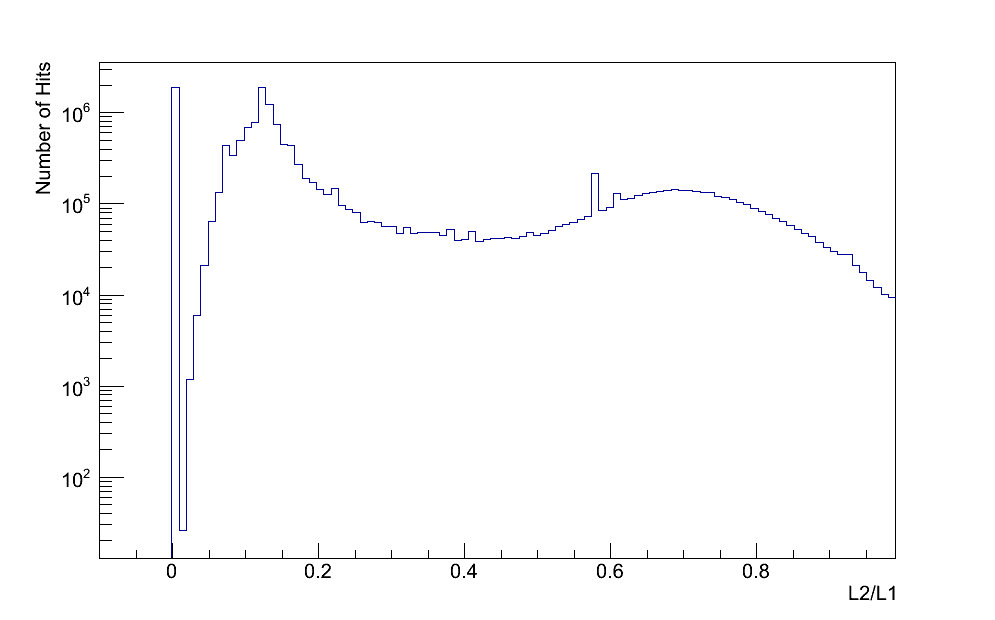
\includegraphics{Hits_Weight}

\caption{\label{fig:Ratio-of-L2/L1}Ratio of L2/L1 derived from PCA of neighbours
hits}


\end{figure}


\begin{figure}


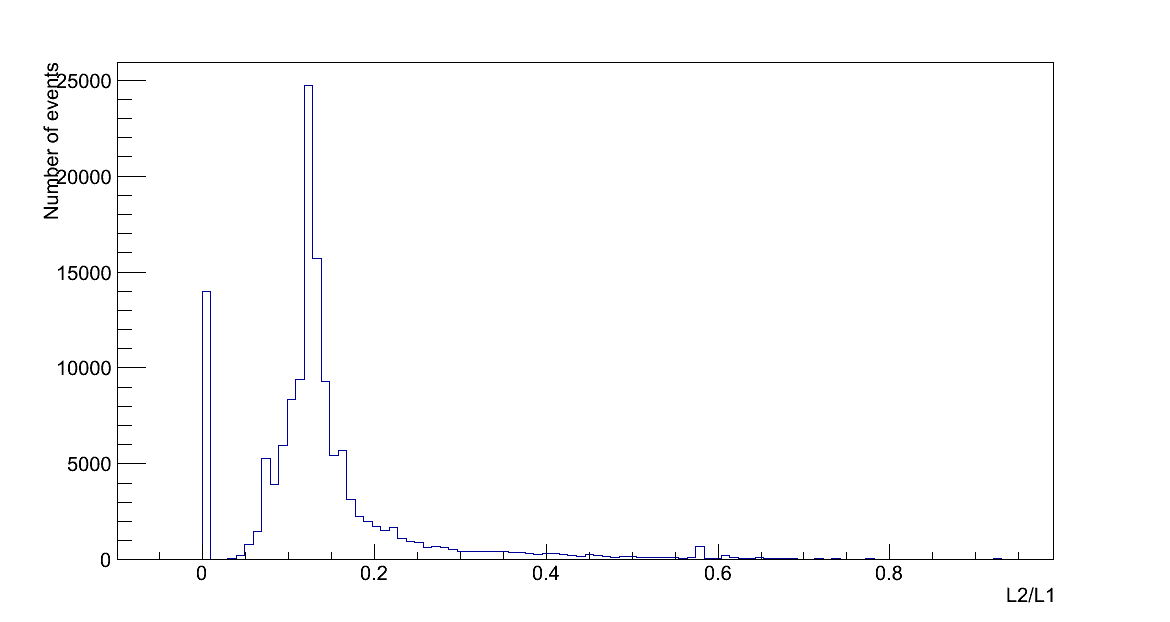
\includegraphics{Hits_Weight_track}\caption{\label{fig:Ratio-of-L2/L1-track}Ratio of L2/L1 for preselected muon
tracks}


\end{figure}

\end{document}
